\documentclass[10pt,a4paper,titlepage]{jreport}

\usepackage[top=25truemm,bottom=25truemm,left=20truemm,right=20truemm]{geometry}
\usepackage[dvipdfmx]{graphicx}
\usepackage{listings,jlisting}

\parindent = 0pt

\lstset{
  basicstyle={\small},
  breaklines=true,
  frame=single,
  tabsize=3,
  numbers=left
}

\title{ データベース 演習課題レポート\\第2回提出}
\author{学生番号: 222C1029\\\\氏名: 江藤 洸陽}
\date{\today}

\begin{document}
\maketitle

\chapter{データベーススキーマの設計}

\section{初期スキーマの作成}
歴代の横綱の情報を管理するためのデータベースを作成する。\\
横綱の情報を表すために必要な属性を書き出して、以下の初期スキーマを作成した。\\
\\
横綱 ( 横綱代位, 出身, 四股名, 部屋番号, 部屋名, 横綱昇進年 )

\subsection{属性の説明}

初期スキーマにおける各属性の役割とドメインは、以下の通りである。

\begin{description}

\item[横綱代位]
横綱の代数を表す。2桁の数字による文字列となる。

\item[出身]
横綱の出身地域を表す。最大4文字の文字列となる。

\item[四股名]
横綱の四股名を表す。最大7文字の文字列となる。
  
\item[部屋番号]
力士が所属する相撲部屋の番号を表す。2桁の数字による文字列となる。

\item[部屋名]
力士が所属する相撲部屋を表す。 最大4文字の文字列となる。

\item[横綱昇進年]
横綱に昇進した年を表す。4桁の数字による文字列となる。

\end{description}

\section{リレーションに格納されるデータ}

横綱リレーションに格納されるデータは、以下の条件を満たす。

\begin{enumerate}
\item 横綱には固有の横綱代位が割り当てられており、横綱代位が同じである横綱が複数存在することはない。
\item 四股名と横綱昇進年の両方が同じ横綱が複数存在することはない。
\item 各部屋には固有の部屋番号を割り当てており、部屋番号が同じである横綱は部屋名も同じとなる。
\end{enumerate}


\subsection{候補キー・主キー}
条件1より、\{ 横綱代位 \} は横綱リレーションの候補キーとなる。\\
条件2より、\{ 四股名, 横綱昇進年\} も横綱リレーションの候補キーとなる。\\
ここでは、2つの候補キーのうち、横綱代位 を主キーとする。\\
主キー属性に下線を引いた初期スキーマは、以下の通りである。\\

横綱( \underline{横綱代位}, 出身, 四股名, 部屋番号, 部屋名, 横綱昇進年 )


\subsection{関数従属性・多値従属性}
条件3 より、部屋番号 → 部屋名 の関数従属性が存在する。\\

\section{リレーションスキーマの正規化}
横綱リレーションが全ての正規形を満たすように、正規化を行う。


\subsection{第1正規形}
横綱レーションは、全ての属性が単一の値を持つため、第1正規形を満たす。\\


\subsection{第2正規形}
横綱リレーションは、候補キーの一部の属性から候補キー以外の属性への関数従属性は存在しないため、第2正規形を満たす。\\

\subsection{第3正規形}
横綱リレーションは、部屋番号 → 部屋名 の関数従属性により、候補キー以外の属性から候補キー以外の属性への関数従属性が存在するため、第3正規形を満たさない。
第3正規形を満たすようにするために、横綱リレーションを、以下のように分解する。\\

横綱( \underline{横綱代位}, 出身, 四股名, 部屋番号, 横綱昇進年)\\
部屋( \underline{部屋番号}, 部屋名)\\

\subsection{ボイス・コッド正規形}
横綱リレーションは、キー属性の一部が非キー属性に関数従属しないのでボイスコット正規形を満たす。\\
部屋リレーションは、キー属性の一部が非キー属性に関数従属しないのでボイスコット正規形を満たす。\\


\subsection{第4正規形}
横綱リレーションは、すべての非キー属性が他の非キー属性に対して完全関数従属しているので第4正規系を満たす。\\
部屋リレーションは、すべての非キー属性が他の非キー属性に対して完全関数従属しているので第4正規系を満たす。\\


\subsection{第5正規形}
横綱リレーションは、結合従属性が存在していないので第5正規系を満たす。\\
部屋リレーションは、結合従属性が存在していないので第5正規系を満たす。\\

\section{正規化後のリレーションスキーマ}
最終的に、以下のリレーションスキーマが得られた。\\

横綱( \underline{横綱代位}, 出身, 四股名, 部屋番号, 横綱昇進年)\\
部屋( \underline{部屋番号}, 部屋名)\\

最終的に得られたリレーションスキーマには、下記の参照整合性制約(外部キー制約)が存在する。\\

横綱の部屋番号(部屋の部屋番号を参照)

\chapter{データベースの作成}

\section{テーブルの定義}
前章で設計した以下のリレーションスキーマにもとづいてデータベースを作成する。\\

横綱( \underline{横綱代位}, 出身, 四股名, 部屋番号, 横綱昇進年 )\\
部屋( \underline{部屋番号}, 部屋名 )\\

参照整合性制約(外部キー制約)\\
横綱の部屋番号(部屋の部屋番号を参照)
\\

テーブル名・属性名をアルファベットに置き換えて、以下のテーブルを作成する。\\

yokozuna( \underline{id}, fro, name, room\_no, promo\_year )\\
room( \underline{room\_no}, name )\\


\section{テーブルの作成}
以下のコマンドを使用して、横綱(yokozuna)テーブルを作成した。

\begin{lstlisting}[caption=横綱テーブルの作成のコマンド]
create table yokozuna(
	id varchar(2) not null unique,
	fro varchar(4),
	name varchar(7) not null,
	room_no varchar(2),
	room varchar(4),
	promo_year varchar(4), 
	primary key( id )
);
\end{lstlisting}
\vspace{3mm}

以下のコマンドを使用して、部屋(room)テーブルを作成した。

\begin{lstlisting}[caption=部屋テーブルの作成のコマンド]
create table room(
	room_no varchar(2) not null unique,
	name varchar(9) not null,
	primary key( room_no )
);
\end{lstlisting}
\vspace{3mm}

以下のコマンドを使用して、横綱(yokozuna)テーブルに参照整合性制約を追加した。

\begin{lstlisting}[caption=横綱テーブルへの参照整合性制約の設定のコマンド]
alter table yokozuna add constraint yokozuna_room_key foreign key (room_no) references room (room_no);
\end{lstlisting}
\vspace{3mm}

以下のコマンドを使用して、全てのテーブルに対して、ウェブサーバへの利用権限を設定した。

\begin{lstlisting}[caption=横綱・部屋テーブルへの利用権限の設定のコマンド]
grant all on yokozuna to apache;
grant all on room to apache;
\end{lstlisting}


\section{初期データの挿入}
以下のテキストファイル・コマンドを使用して、横綱(yokozuna)テーブルに初期データを挿入した。

\begin{lstlisting}[caption=横綱テーブルの初期データ(yokozuna\_data.txt\_list.php)]
63, 青森, 旭富士正也, 02 ,大島 ,1990
64, アメリカ, 曙太郎, 09 ,東関 ,1993
65, 東京, 貴乃花光司, 05 ,二子山 ,1995
66, 東京, 若乃花勝, 05 ,二子山 ,1998
67, アメリカ, 武蔵丸光洋 ,07 , 武蔵川 ,1999
68, モンゴル, 朝青龍明徳 ,03 , 高砂 ,2003
69, モンゴル, 白鵬翔 ,06 ,宮城野 , 2007
70, モンゴル, 日馬富士公平 ,01 ,伊勢ヶ濱 , 2012
71, モンゴル, 鶴竜力三郎 ,08 ,井筒 , 2014
72, 茨城, 稀勢の里寛 ,04 ,田子ノ浦 ,2017

\end{lstlisting}

\begin{lstlisting}[caption=横綱テーブルへの初期データの挿入]
	COPY yokozuna FROM 'yokozuna_data.txt' USING DELIMITERS '.'
\end{lstlisting}
\vspace{3mm}

以下のテキストファイルとコマンドを使用して、部屋(room)テーブルに初期データを挿入した。

\begin{lstlisting}[caption=部屋テーブルへの初期データの挿入(room\_data.txt)]
insert into room values( '01', '伊勢ヶ濱' );
insert into room values( '02', '大島' );
insert into room values( '03', '高砂' );
insert into room values( '04', '田子ノ浦' );
insert into room values( '05', '二子山' );
insert into room values( '06', '宮城野' );
insert into room values( '07', '武蔵川' );
insert into room values( '08', '井筒' );
insert into room values( '09', '東関' );
\end{lstlisting}

\begin{lstlisting}[caption=部屋テーブルへの初期データの挿入]
\i room_data.txt
\end{lstlisting}


\section{テーブルの格納データの確認}
SQLを使って横綱(yokozuna)テーブルに格納されている全てのデータを表示すると、以下のようになる。

\begin{verbatim}
agdo2465=> select * from yokozuna;
 id |   fro    |     name     | room_no |   room   | promo_year
----+----------+--------------+---------+----------+------------
 63 | 青森     | 旭富士正也   | 02      | 大島     | 1990
 64 | アメリカ | 曙太郎       | 09      | 東関     | 1993
 65 | 東京     | 貴乃花光司   | 05      | 二子山   | 1995
 66 | 東京     | 若乃花勝     | 05      | 二子山   | 1998
 67 | アメリカ | 武蔵丸光洋   | 07      | 武蔵川   | 1999
 68 | モンゴル | 朝青龍明徳   | 03      | 高砂     | 2003
 69 | モンゴル | 白鵬翔       | 06      | 宮城野   | 2007
 70 | モンゴル | 日馬富士公平 | 01      | 伊勢ヶ濱 | 2012
 71 | モンゴル | 鶴竜力三郎   | 08      | 井筒     | 2014
 72 | 茨城     | 稀勢の里寛   | 04      | 田子ノ浦 | 2017
 73 | モンゴル | 照ノ富士春雄 | 01      | 伊勢ヶ濱 | 2021
(11 rows)
\end{verbatim}
\vspace{3mm}

SQLを使って部屋(room)テーブルに格納されている全てのデータを表示すると、以下のようになる。

\begin{verbatim}
agdo2465=> select * from room;
 room_no |   name
---------+----------
 01      | 伊勢ヶ濱
 02      | 大島
 03      | 高砂
 04      | 田子ノ浦
 05      | 二子山
 06      | 宮城野
 07      | 武蔵川
 08      | 井筒
 09      | 東関
(9 rows)
\end{verbatim}
\vspace{3mm}


\chapter{データベースへの問い合わせ}

2章で作成したデータベースに対して、以下のようなSQLを使った問い合わせのテストを行った。

\section{問い合わせ1}

問い合わせ:\\
全ての横綱の代数、氏名、部屋、出身の一覧を出力する。\\

SQL:
\begin{verbatim}
select id, yokozuna.name, room.name, yokozuna.fro from yokozuna, room 
where yokozuna.room_no = room.room_no
\end{verbatim}
\vspace{3mm}

実行結果:
\begin{verbatim}
abcd1234=>  select id, yokozuna.name, room.name, fro from yokozuna, room
where yokozuna.room_no = room.room_no;
 id |     name     |   name   |   fro
----+--------------+----------+----------
 63 | 旭富士正也   | 大島     | 青森
 64 | 曙太郎       | 東関     | アメリカ
 65 | 貴乃花光司   | 二子山   | 東京
 66 | 若乃花勝     | 二子山   | 東京
 67 | 武蔵丸光洋   | 武蔵川   | アメリカ
 68 | 朝青龍明徳   | 高砂     | モンゴル
 69 | 白鵬翔       | 宮城野   | モンゴル
 70 | 日馬富士公平 | 伊勢ヶ濱 | モンゴル
 71 | 鶴竜力三郎   | 井筒     | モンゴル
 72 | 稀勢の里寛   | 田子ノ浦 | 茨城
 73 | 照ノ富士春雄 | 伊勢ヶ濱 | モンゴル
(11 rows)
\end{verbatim}


\section{問い合わせ2}

問い合わせ:\\
横綱の代が'73'の横綱と同じ部屋に所属する横綱の、横綱代数と四股名の一覧を出力する。\\

SQL:
\begin{verbatim}
select id, name from yokozuna
where room_no = (select room_no from yokozuna where id = '73');
\end{verbatim}
\vspace{3mm}

実行結果:
\begin{verbatim}
 id |     name
----+--------------
 70 | 日馬富士公平
 73 | 照ノ富士春雄
(2 rows)
\end{verbatim}


\section{問い合わせ3}

問い合わせ:\\
各部屋で最も横綱になったのが遅かった人を検索して、各部屋の部屋名、部屋内の該当者の四股名、年の一覧を出力する。\\

SQL:
\begin{verbatim}
select id, name, room, promo_year
from yokozuna 
where (room, promo_year) in (
	select room, max(promo_year) as max_year
	from yokozuna
	group by room
)
order by room;
\end{verbatim}

実行結果:
\begin{verbatim}
  id |     name     |   room   | promo_year
----+--------------+----------+------------
	66 | 若乃花勝     | 二子山   | 1998
	71 | 鶴竜力三郎   | 井筒     | 2014
	73 | 照ノ富士春雄 | 伊勢ヶ濱 | 2021
	63 | 旭富士正也   | 大島     | 1990
	69 | 白鵬翔       | 宮城野   | 2007
	64 | 曙太郎       | 東関     | 1993
	67 | 武蔵丸光洋   | 武蔵川   | 1999
	72 | 稀勢の里寛   | 田子ノ浦 | 2017
	68 | 朝青龍明徳   | 高砂     | 2003
(9 rows)
\end{verbatim}


\chapter{Webインターフェースの作成}

\section{作成したインターフェースのメニューページ}



2章で作成したデータベースを利用するためのインターフェースを開発した。\\
作成したインターフェースのメニューページのURLは、下記の通りである。

\begin{verbatim}
http://db.tom.ai.kyutech.ac.jp/~agdo2465/menu.html
\end{verbatim}


\section{作成したインターフェースの構成}

横綱と部屋を結合して一覧表示する機能を作成した。\\
横綱テーブルへのデータの挿入・削除・更新のための機能を作成した。\\
部屋テーブルについては、更新の頻度が少ないため、データの挿入・削除・更新の機能は作成していない。\\
また、横綱を部屋と出身と横綱昇進年の条件を組み合わせて検索できる機能を作成した。\\
インターフェースを構成するファイルの役割や階層構造は、下記の通りである

\begin{itemize}
\item メニューページ(menu.html)
	\begin{itemize}
	\item 横綱・部屋の一覧表示(yokozuna\_list.php)
	\item 横綱のデータ追加の入力フォーム(yokozuna\_add\_form.php)
		\begin{itemize}
			\item 横綱のデータ追加の処理実行(yokozuna\_add.php)
		\end{itemize}
	\item 横綱のデータ削除の選択(yokozuna\_delete\_form.php)
		\begin{itemize}
			\item 横綱のデータ削除の処理実行(yokozuna\_delete.php)
		\end{itemize}
	\item 横綱のデータ更新の選択(yokozuna\_update\_form1.php)
		\begin{itemize}
			\item 横綱のデータ更新の入力フォーム(yokozuna\_update\_form2.php)
			\begin{itemize}
				\item 横綱のデータ更新の処理実行(yokozuna\_update.php)
			\end{itemize}
		\end{itemize}
	\item 横綱の検索の入力フォーム(yokozuna\_search\_form.php)
		\begin{itemize}
			\item 横綱の検索結果の表示(yokozuna\_search\_result.php)
		\end{itemize}
	\end{itemize}
\end{itemize}


\section{メニューページ}

メニューページは、上記の階層構造においてメニューページの下位のページである、横綱・横綱の一覧表示(yokozuna\_list.php)、横綱のデータ追加(yokozuna\_add\_form.php)、横綱のデータ削除(yokozuna\_delete\_form.php)、横綱のデータ更新(yokozuna\_update\_form1.php)、横綱の検索(yokozuna\_search\_form.php)の各ページへのリンクを含む。

\lstinputlisting[caption=menu.html]{menu.html}

図\ref{fig:menu} は、ウェブブラウザでメニューページを表示したときのスクリーンショットを示したものである。

\begin{figure}[h]
	\begin{center}
		\fbox{
			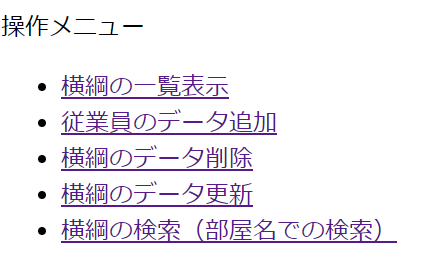
\includegraphics[width=0.4\textwidth]{menu1.png}
		}
	\end{center}
	\caption{メニューページの表示結果
	}
	\label{fig:menu}
\end{figure}


\section{横綱の一覧表示}

\subsection{横綱の一覧表示(yokozuna\_list.php)}

全横綱の一覧を表示するPHPプログラムを含むページである。横綱と部屋のテーブルを結合して、横綱代数にもとづいて昇順で並べて表示する。また、全体で何件の横綱のデータが存在しているかの情報を、横綱一覧の後に表示する。\\

プログラムの27行目で横綱の一覧を作成するSQL文を作成して、30行目でそのSQL文を実行している。\\

\begin{lstlisting}[caption=横綱の一覧表示のためのSQL]
select id, room.name, yokozuna.name, fro, promo_year from yokozuna, room where yokozuna.room_no = room.room_no order by id
\end{lstlisting}

この問い合わせは、前ページでの利用者の入力によって変化するようなことはなく、毎回同じ問い合わせを実行するため、ソースファイル中で固定のSQL文を文字列として設定している。

\lstinputlisting[caption=yokozuna\_list.php]{yokozuna_list.php}


\subsection{横綱の一覧表示の実行例}

図\ref{fig:example_list1} は、一覧表示の操作を行ったときのスクリーンショットを示したものである。

\begin{figure}[h]
	\begin{center}
		\fbox{
			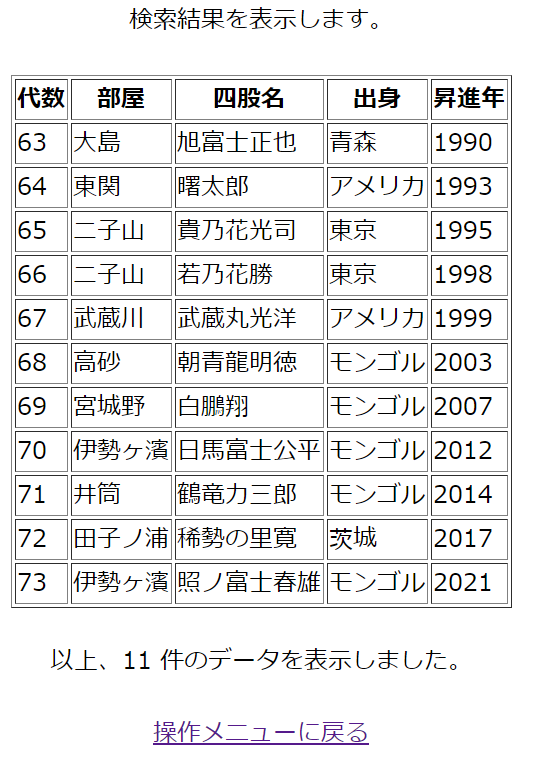
\includegraphics[width=0.4\textwidth]{yokozuna_list.png}
		}
	\end{center}
	\caption{横綱の一覧表示の実行結果
	}
	\label{fig:example_list1}
\end{figure}


\section{横綱の追加}


\subsection{横綱のデータ追加の入力フォーム(yokozuna\_add\_form.php)}

横綱のデータを追加するPHPプログラムを含むページである。横綱代数、部屋、四股名、横綱昇進年、出身を入力して、追加する。また、部屋については選択式にしている。
プログラムの28行目で横綱の一覧を作成するSQL文を作成して、30行目でそのSQL文を実行している。\\

\lstinputlisting[caption=yokozuna\_add\_form.php]{yokozuna_add_form.php}

\subsection{横綱のデータ追加の処理実行(yokozuna\_add.php)}

前のページのフォームに対して入力された、以下の情報を受け取る。プログラムの12~16行目で、これらのデータを取得して、各変数に代入する。

\lstinputlisting[caption=yokozuna\_add.php]{yokozuna_add.php}

\begin{itemize}
\item 横綱代数(id) → \$id
\item 部屋番号(room\_no) → \$room\_no
\item 氏名(name) → \$name
\item 年齢(fro) → \$fro
\item 横綱昇進年(promo\_year) →\$promo\_year
\end{itemize}

プログラムの30行目で、横綱テーブルにインスタンスを追加するためのSQL文を作成する。
SQL文の \%1, \%2, \%3, \%4, \%5 には、変数 \$id, \$room\_no, \$name, \$fro, \$promo\_year の値が挿入される。
38行目で、作成したSQL文を実行する。\\

\begin{lstlisting}[caption=横綱の追加のためのSQL]
insert into yokozuna values( %1, %2, %3, %4, %5 )
\end{lstlisting}
\vspace{3mm}


\subsection{横綱の追加の実行例}

図\ref{fig:example_list2} は、データ追加をする画面のスクリーンショットを示したものである。

\begin{figure}[h]
	\begin{center}
		\fbox{
			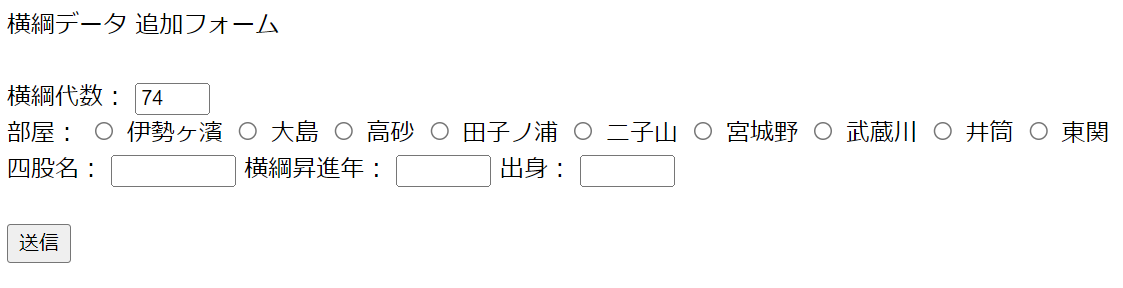
\includegraphics[width=0.4\textwidth]{yokozuna_add.png}
		}
	\end{center}
	\caption{横綱の一覧表示の実行結果
	}
	\label{fig:example_list2}
\end{figure}


\section{横綱の削除}


\subsection{横綱のデータ削除の選択(yokozuna\_delete\_form.php)}

横綱のデータを削除するPHPプログラムを含むページである。横綱代数、部屋、四股名、横綱昇進年、出身が表示されてる画面で、横綱代数を選択して、削除する。
プログラムの30行目で横綱の一覧を作成するSQL文を作成して、33行目でそのSQL文を実行している。\\

\lstinputlisting[caption=yokozuna\_delete\_form.php]{yokozuna_delete_form.php}


\subsection{横綱のデータ削除の処理実行(yokozuna\_delete.php)}

前のページのフォームに対して入力された、以下の情報を受け取る。プログラムの12行目で、これらのデータを取得して、各変数に代入する。

\lstinputlisting[caption=yokozuna\_delete.php]{yokozuna_delete.php}

\begin{itemize}
\item 横綱代数(id) → \$id
\end{itemize}

プログラムの26行目で、横綱テーブルからインスタンスを削除するためのSQL文を作成する。
34行目で、作成したSQL文を実行する。\\

\begin{lstlisting}[caption=横綱の削除のためのSQL]
delete from yokozuna where id = '%s' 
\end{lstlisting}
\vspace{3mm}

\subsection{横綱の削除の実行例}

図\ref{fig:example_list3} は、データ追加をする画面のスクリーンショットを示したものである。

\begin{figure}[h]
	\begin{center}
		\fbox{
			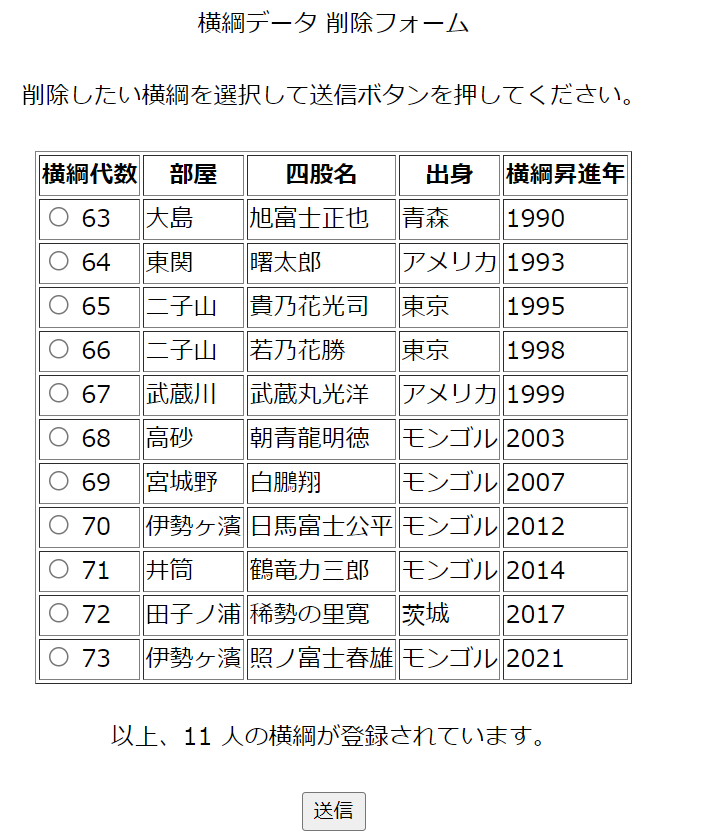
\includegraphics[width=0.4\textwidth]{yokozuna_delete.png}
		}
	\end{center}
	\caption{横綱の一覧表示の実行結果
	}
	\label{fig:example_list3}
\end{figure}


\section{横綱の更新}


\subsection{横綱のデータ更新の選択(yokozuna\_update\_form1.php)}

横綱のデータを更新するPHPプログラムを含むページである。横綱代数、部屋、四股名、横綱昇進年、出身が表示されてる画面で、横綱代数を選択する。
プログラムの31行目で横綱の一覧を作成するSQL文を作成して、34行目でそのSQL文を実行している。\\

\lstinputlisting[caption=yokozuna\_update\_form1.php]{yokozuna_update_form1.php}


\subsection{横綱のデータ更新の入力フォーム(yokozuna\_update\_form2.php)}

横綱のデータを更新するPHPプログラムを含むページである。データを追加するときと似たような画面で、部屋以外は既に入力されているものから編集できる。しかしながら、代数は変えることができない。
プログラムの31行目で横綱の一覧を作成するSQL文を作成して、34行目でそのSQL文を実行している。\\

\lstinputlisting[caption=yokozuna\_update\_form2.php]{yokozuna_update_form2.php}


\subsection{横綱のデータ更新の処理実行(yokozuna\_update.php)}

前のページのフォームに対して入力された、以下の情報を受け取る。プログラムの48行目で、これらのデータを取得して、各変数に代入する。

\lstinputlisting[caption=yokozuna\_update.php]{yokozuna_update.php}

\begin{itemize}
	\item 横綱代数(id) → \$id
	\item 氏名(name) → \$name
	\item 年齢(fro) → \$fro
	\item 横綱昇進年(promo\_year) →\$promo\_year
	\end{itemize}

プログラムの30行目で、横綱テーブルからインスタンスを変更するためのSQL文を作成する。
SQL文の \%1, \%2, \%3, \%4, \%5 には、変数 \$id, \$room\_no, \$name, \$fro, \$promo\_year の値が挿入される。
33行目で、作成したSQL文を実行する。\\

\begin{lstlisting}[caption=横綱の更新のためのSQL]
	update yokozuna set(%1, %2, %3, %4, %5)
\end{lstlisting}
\vspace{3mm}


\subsection{横綱のデータ更新の実行例}

図\ref{fig:yokozuna_update1}~\ref{fig:yokozuna_update5} は、横綱「白鳳」の出身を「モンゴル」から「モザンピーク」に更新する操作を行ったときの、一連のスクリーンショットを示したものである。

\begin{figure}[h]
	\begin{center}
		\fbox{
			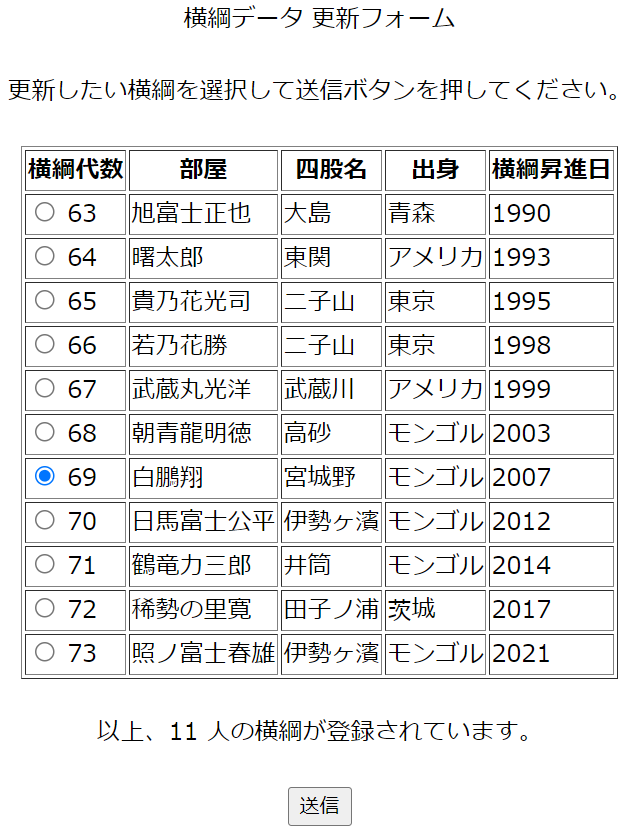
\includegraphics[width=0.6\textwidth]{yokozuna_update1.png}
		}
	\end{center}
	\caption{横綱の更新の実行結果(1):選択フォームから更新する横綱を選択
	}
	\label{fig:yokozuna_update1}
\end{figure}

\begin{figure}[h]
	\begin{center}
		\fbox{
			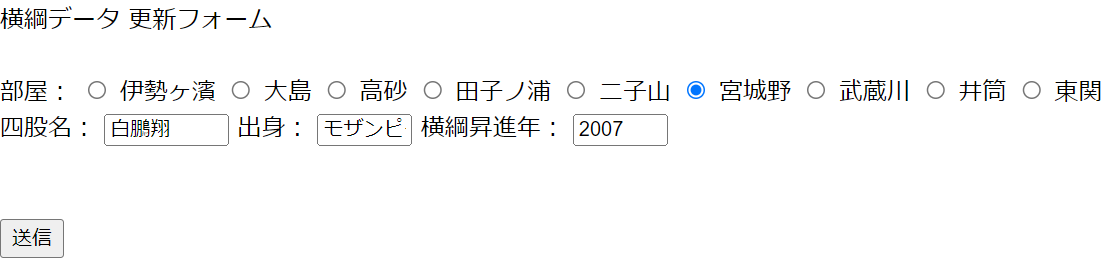
\includegraphics[width=0.6\textwidth]{yokozuna_update2.png}
		}
	\end{center}
	\caption{横綱の更新の実行結果(2):入力フォームに移り、選択した横綱の現在の情報が表示される
	}
	\label{fig:yokozuna_update2}
\end{figure}

\begin{figure}[h]
	\begin{center}
		\fbox{
			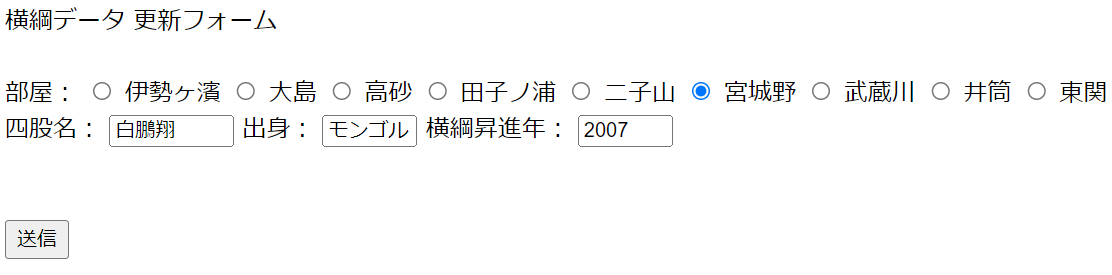
\includegraphics[width=0.6\textwidth]{yokozuna_update3.png}
		}
	\end{center}
	\caption{横綱の更新の実行結果(3):入力フォームで、横綱の情報を変更して、送信ボタンを押す
	}
	\label{fig:yokozuna_update3}
\end{figure}

\begin{figure}[h]
	\begin{center}
		\fbox{
			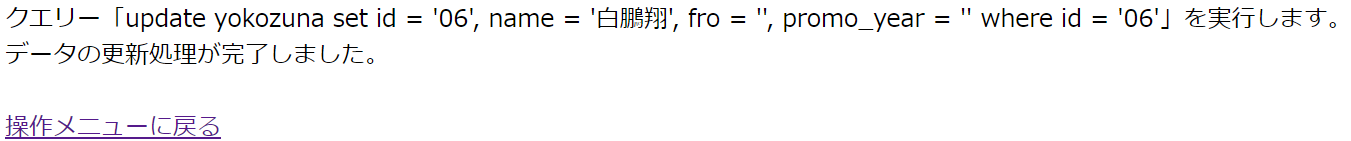
\includegraphics[width=0.8\textwidth]{yokozuna_update4.png}
		}
	\end{center}
	\caption{横綱の更新の実行結果(4):更新処理の実行結果が表示される
	}
	\label{fig:yokozuna_update4}
\end{figure}

\begin{figure}[h]
	\begin{center}
		\fbox{
			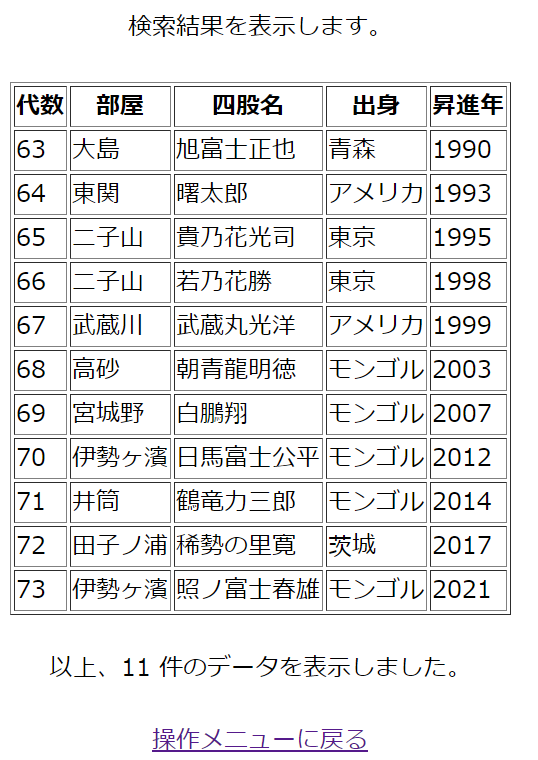
\includegraphics[width=0.8\textwidth]{yokozuna_update5.png}
		}
	\end{center}
	\caption{横綱の更新の実行結果(5):更新処理の実行結果が表示される
	}
	\label{fig:yokozuna_update5}
\end{figure}

\clearpage

\section{横綱の検索}


\subsection{横綱の検索の入力フォーム(yokozuna\_search\_form.php)}

\lstinputlisting[caption=yokozuna\_search\_form.php]{yokozuna_search_form.php}

\subsection{横綱の検索結果の表示(yokozuna\_search\_result.php)}

\lstinputlisting[caption=yokozuna\_search.php]{yokozuna_search.php}

横綱の検索
前のページのフォームに対して入力された、以下の情報を受け取る。プログラムの??行目で、データを取得して、変数に代入する。

\begin{itemize}
\item 部屋(room\_no) → \$room\_no
\end{itemize}

プログラムの30~33行目で、横綱の検索を行うためのSQL文を作成する。
変数 \$room\_no に文字列「ALL」が格納されている場合は、全ての横綱の横綱を表示するためのSQLを実行する。

\begin{lstlisting}[caption=全ての横綱を表示するためのSQL]
select id, room.name, yokozuna.name, fro, promo_year from yokozuna, room where yokozuna.room_no = room.room_no order by id";
\end{lstlisting}
\vspace{3mm}

変数 \$room\_no に「ALL」以外の文字列が格納されている場合は、部屋番号が \$room\_no に等しい横綱のみを表示するためのSQLを実行する。
SQL文の \$\_room には、その変数の値が挿入される。

\begin{lstlisting}[caption=指定された部屋番号に所属する横綱を検索するためのSQL]
select id, room.name, yokozuna.name, fro, promo_year from yokozuna, room where yokozuna.room_no = room.room_no and yokozuna.room_no = '$room_no' order by id";
\end{lstlisting}
\vspace{3mm}


\subsection{横綱のデータ検索の実行例}


図\ref{fig:yokozuna_search1}~\ref{fig:yokozuna_search2} は、横綱のみを条件とする検索の実行例として、部屋が「二子山」である横綱を検索する操作を行ったときの、一連のスクリーンショットを示したものである。\\

\begin{figure}[h]
	\begin{center}
		\fbox{
			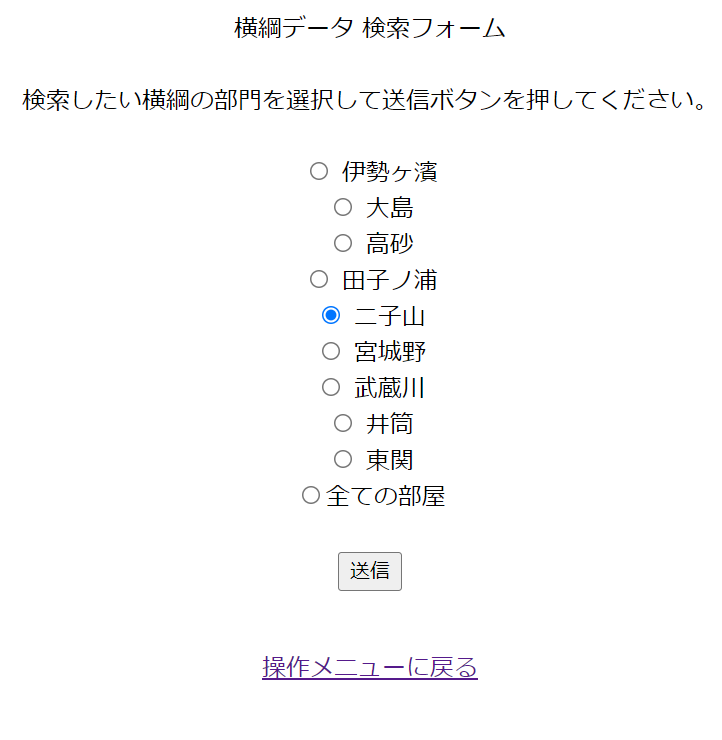
\includegraphics[width=0.8\textwidth]{yokozuna_search1.png}
		}
	\end{center}
	\caption{横綱の検索の実行結果(1):選択フォームから検索する横綱を選択
	}
	\label{fig:yokozuna_search1}
\end{figure}

\begin{figure}[h]
	\begin{center}
		\fbox{
			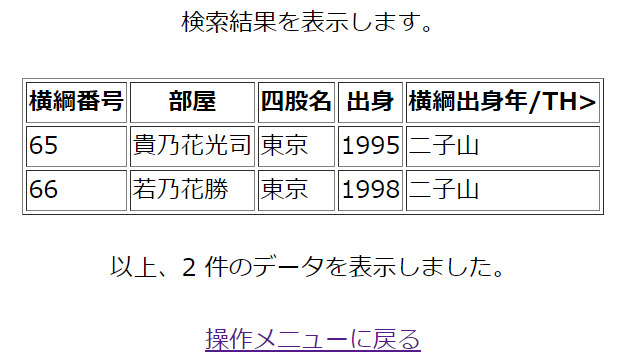
\includegraphics[width=0.8\textwidth]{yokozuna_search2.png}
		}
	\end{center}
	\caption{横綱の検索の実行結果(2):出力フォームに移り、検索した横綱の情報が表示される
	}
	\label{fig:yokozuna_search2}
\end{figure}


\chapter{まとめ}

とても大変でした。

\end{document}